% 冷原子基本知识
% 冷原子|能级|角动量|碱金属|原子结构

研究冷原子主要是两方面(其中后者更重要):原子的内部结构,和原子原子之间的相互作用.

首先研究原子内部结构,我们可以先写出单原子的 Hamiltonian,
\begin{equation}
\begin{split}
\hat{H}_{at}=&-\sum_i\left(\frac{\hbar^2\nabla_i^2}{2\mu_i}+V_{ei}({\bvec r})\right) + \sum_{i<j}V_{ee}({\bvec r}_i-{\bvec r}_j)\\
&+\sum_i [\alpha_f {\bvec S}_i\cdot{\bvec L}_i+\alpha_{hf}({\bvec S}_i+{\bvec L}_i)\cdot {\bvec I}_i]
\end{split}
\end{equation}

如果只考虑第一项,也就是说每个电子之间是没有相互作用的,得到的是很经典的能级,我们中学就学过. 第二项的作用是给了一个修正,当然一般的表达式并不容易写出来,但是我们知道能量的修正可以写成如下形式
\begin{equation}
E = -\frac{\mu\alpha^2}{2\hbar^2(n+\Delta)^2},\quad \Delta = \Delta(n,l),\quad \alpha = \frac{e^2}{4\pi\varepsilon_0}
\end{equation}

除此之外,第二项还能提供一个我们所知的Hund规则,单重态 $\psi_1({\bvec r}_1)\psi_2({\bvec r}_2)-\psi_1({\bvec r}_2)\psi_2({\bvec r}_1)$ 在离的很近的时候波函数是基本没有的,也就是提供了一个repulsive的能量;这也就是说三重态相比单重态能量更低.

第三项,正如他的名字所暗示的,包含着精细结构(fine)和超精细结构(hyperfine)

原子物理里面,一个很基本的概念就是Zeeman效应,这是实验上观测到,并在后来基于量子理论建立了正确的描述;很通俗而且愚蠢的Zeeman项(系数)的解释是:相对的,原子核(带电)绕电子转圈,引发磁场,与电子的自旋相互作用.
\begin{equation}
E\propto -{\bvec\mu}_s\cdot{\bvec B}_{\text{eff}}=\frac{Ze^2\mu_0}{8\pi m_0^2 r^3}({\bvec S\cdot L})
\end{equation}

这一项相比与之前大概是 $10^{-3}$的量级;而电子整体的角动量与核自旋的相互作用是超精细结构,相比精细结构是$10^{-3}$ 的量级.

物理学对原子进行分类,主要有三类(实际上有很多更精细的分化,但在冷原子范畴内我们并不关心原子形成的晶体的结构:我们希望在极低温度的情况下,原子仍然能保证不会结晶而是气态;这也是冷原子的密度极低,十分稀薄从而少体散射就适用的一个原因):

碱金属:锂钠钾铷铯钫. $^{2S+1}L_J$ 表示的话,这些原子的基态都是 $^2 S_{1/2}$,价电子都是 $ns^1$,区别主要体现在核自旋上(不同的同位素). $^{87}\text{Rb}, ^{23}\text{Na}$ 是最常见最爱研究的玻色气体,而 $^{40}\text{K}, ^6 \text{Li}$ 则是最常见的费米气体. Fermion or Boson 主要看核自旋是整数还是半整数.

作为例子看一个问题:

$^{87}{\text{Rb}}, ^6{\text{Li}}$ 在磁场 $\bvec B = B\uvec z$ 中,Hamiltonian可以写成
\begin{equation}
\hat{H} = B(\mu_B J_z+\mu_N I_z)+\alpha({\bvec J\cdot I})
\end{equation}

这个的处理方法实际上和传统的 $LS$ 耦合基本一样:引入一个新的参数 ${\bvec F = J+I}$,从而保证
\begin{equation}
{\bvec J\cdot I} = \frac{1}{2}({\bvec F}^2 - {\bvec J}^2 - {\bvec I}^2) = \frac{1}{2} (F(F+1) - J(J+1) - I(I+1))
\end{equation}

从而能谱就是
\begin{equation}
E = B(\mu_B J_z+\mu_N I_z)+\frac{\alpha}{2} (F(F+1) - J(J+1) - I(I+1))
\end{equation}

除此之外,我们还可以看到另外的东西. 这个 Hamiltonian 不好解,但是我们可以用 $|F,m_F\rangle$ 来展开,并且把超精细结构的项作为perturbation来处理. $^{87}{\text{Rb}}: I = \frac{3}{2};\ ^6{\text{Li}}: I = 1; J = \frac{1}{2}$

对于 $^{87}{\text{Rb}}$ 来说,能够得到的 $F=2,1$. 其本征态有两系列
$F=2:|2,0\rangle,|2,\pm1\rangle,|2,\pm2\rangle$
$F=1:|1,0\rangle,|1,\pm1\rangle$

但是我们知道, $|F,m_F\rangle$ 必须利用 $CG$ 系数知道它实际上是如何被组合成的,才能用我们的Hamiltonian计算.

\begin{align}
&\ket{2,2} = \ket{\frac{3}{2},\frac{3}{2}} \ket{\frac{1}{2},\frac{1}{2}}\\
&\ket{2,1} = \frac{1}{2} \ket{\frac{3}{2},\frac{3}{2}} \ket{\frac{1}{2},-\frac{1}{2}} + \frac{\sqrt{3}}{2} \ket{\frac{3}{2},\frac{1}{2}} \ket{\frac{1}{2},\frac{1}{2}}\\
& \ket{2,0} = \frac{\sqrt{2}}{2} \ket{\frac{3}{2},\frac{1}{2}} \ket{\frac{1}{2},-\frac{1}{2}} + \frac{\sqrt{2}}{2} \ket{\frac{3}{2},-\frac{1}{2}} \ket{\frac{1}{2},\frac{1}{2}}\\
&\ket{2,-1} = \frac{1}{2} \ket{\frac{3}{2},-\frac{3}{2}} \ket{\frac{1}{2},\frac{1}{2}} + \frac{\sqrt{3}}{2} \ket{\frac{3}{2},-\frac{1}{2}} \ket{\frac{1}{2},-\frac{1}{2}}\\
& \ket{2,-2} = \ket{\frac{3}{2},-\frac{3}{2}} \ket{\frac{1}{2},-\frac{1}{2}}\\
&\ket{1,1} = \frac{\sqrt{3}}{2} \ket{\frac{3}{2},\frac{3}{2}} \ket{\frac{1}{2},-\frac{1}{2}} - \frac{1}{2} \ket{\frac{3}{2},\frac{1}{2}} \ket{\frac{1}{2},\frac{1}{2}}\\
&\ket{1,0} = \frac{\sqrt{2}}{2} \ket{\frac{3}{2},\frac{1}{2}} \ket{\frac{1}{2},-\frac{1}{2}} - \frac{\sqrt{2}}{2} \ket{\frac{3}{2},-\frac{1}{2}} \ket{\frac{1}{2},\frac{1}{2}}\\
&\ket{1,-1} = -\frac{\sqrt{3}}{2} \ket{\frac{3}{2},-\frac{3}{2}} \ket{\frac{1}{2},\frac{1}{2}} + \frac{1}{2} \ket{\frac{3}{2},-\frac{1}{2}} \ket{\frac{1}{2},-\frac{1}{2}}
\end{align}

这样写出来的Hamiltonian是一个 $8\times8$ 的矩阵,当然大部分矩阵元都是 0,但是对角项和一些部分也不是 $0$. 利用一些技巧,我们知道只有拥有同样的 $m_F$ 的两个态之间才有矩阵元,凭借惊人的毅力,我们把这个矩阵写出来,如\autoref{UCBas_fig1}(本人的计算功底很差\ldots 如果算错了不要打我\footnote{注意:确实发现算错了,但是懒得改,领会精神orz}):

\begin{figure}[ht]
\centering
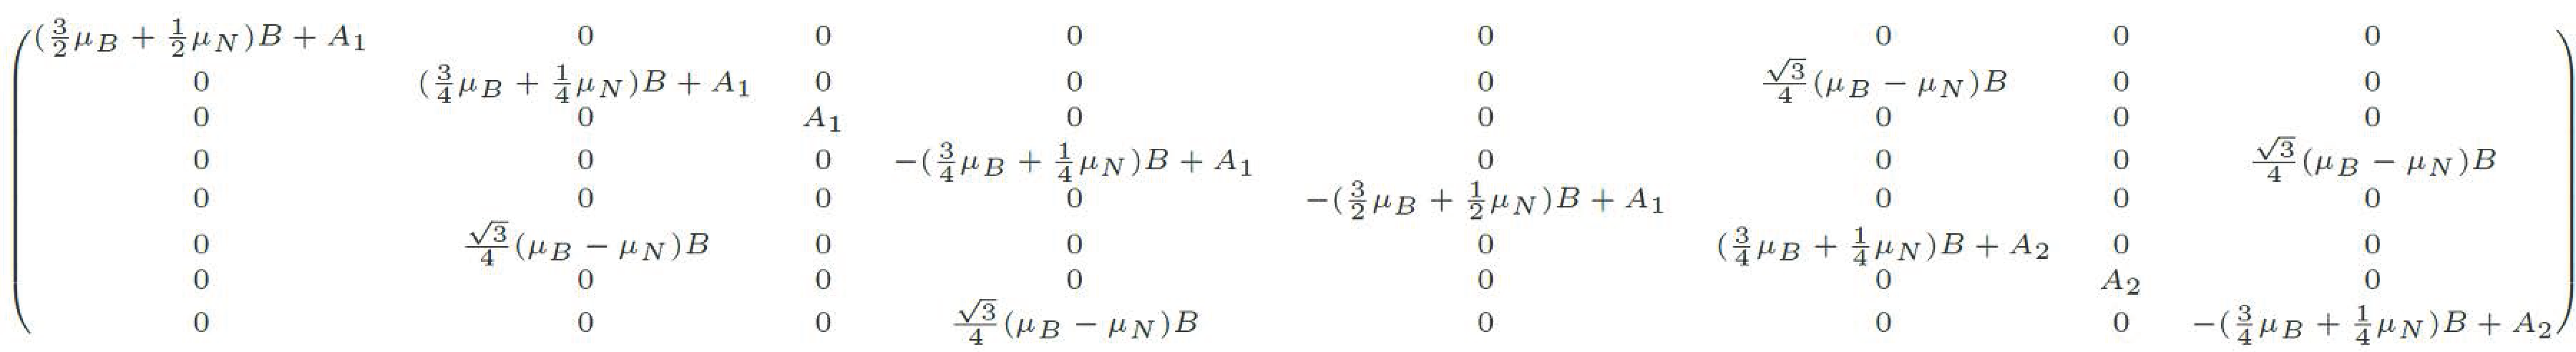
\includegraphics[width=15cm]{./figures/UCBas_1.png}
\caption{算错的矩阵} \label{UCBas_fig1}
\end{figure}

\begin{equation}\ali{
&A_1\equiv\frac{3}{4}\alpha = \frac{\alpha}{2}\left(2\times3 - \frac{3}{2}\times\frac{5}{2} - \frac{1}{2}\times\frac{3}{2}\right)\\
&A_2 \equiv -\frac{5}{4}\alpha = \frac{\alpha}{2}\left(1\times2 - \frac{3}{2}\times\frac{5}{2} - \frac{1}{2}\times\frac{3}{2}\right)
}\end{equation}

发现,只有在 $|2,1\rangle,|1,1\rangle$ 和 $|2,-1\rangle,|1,-1\rangle$ 之间存在off-diagonal成分. 相当于我们需要对角化如下两个 $2\times$ 矩阵:
\begin{equation}\ali{
\left(
\begin{matrix}
\left(\frac{3}{4}\mu_B+\frac{1}{4}\mu_N\right)B+A_1 & \frac{\sqrt{3}}{4}(\mu_B-\mu_N)B\\
\frac{\sqrt{3}}{4}(\mu_B-\mu_N)B & \left(\frac{3}{4}\mu_B+\frac{1}{4}\mu_N\right)B+A_2
\end{matrix}
\right),\\
\left(
\begin{matrix}
-\left(\frac{3}{4}\mu_B+\frac{1}{4}\mu_N\right)B+A_1 & \frac{\sqrt{3}}{4}(\mu_B-\mu_N)B\\
\frac{\sqrt{3}}{4}(\mu_B-\mu_N)B & -\left(\frac{3}{4}\mu_B+\frac{1}{4}\mu_N\right)B+A_2
\end{matrix}
\right)
}\end{equation}

得到这两部分的本征值分别应该为
\begin{equation}
\lambda_{1,2/1} = -\left(\frac{3}{4}\mu_B-\frac{1}{4}\mu_N\right)B+\frac{A_1+A_2}{2} \pm \sqrt{\frac{1}{4}(A_1-A_2)^2+\frac{3}{4}(\mu_B-\mu_N)^2B^2}
\end{equation}
\begin{equation}
\lambda_{-1,2/1} = \left(\frac{3}{4}\mu_B+\frac{1}{4}\mu_N\right)B+\frac{A_1+A_2}{2} \pm \sqrt{\frac{1}{4}(A_1-A_2)^2+\frac{3}{4}(\mu_B-\mu_N)^2B^2}
\end{equation}

这两个本征值的行为在 $B$ 非常小和相对大一点的时候有着截然不同的表现. 在很小的时候,也就是说 $B\ll|A_1-A_2| / \sqrt{3}(\mu_B-\mu_N)$,我们可以把根号内进行展开,得到
\begin{equation}
\sqrt{\frac{1}{4}(A_1-A_2)^2+\frac{3}{4}(\mu_B-\mu_N)^2B^2} \approx \frac{1}{2}|A_1-A_2| \qty(1+\frac{3}{2}\frac{(\mu_B-\mu_N)^2}{(A_1-A_2)^2}B^2)
\end{equation}

得到了一个Zeeman \text{eff}ect的二次shift. 而大的磁场下超精细结构 $A_1, A_2$ 很小,几乎忽略,主要修正项都是 $\frac{\sqrt{3}}{2}\Delta\mu B$,是线性的 Zeeman shift.

当然这只是一个关于二次Zeeman shift的例子,$^6{\text{Li}}$ 同理,有兴趣的同学可以进行练习.

碱金属原子的另一个特点就是明显的第一激发态的劈裂. 第一激发态本身应该是 $L=1$,也就是 $^2P$. 但是如果有了 $LS$ 耦合,不同的 $J$ 会有不同的精细结构劈裂. 最简单的就是大家都实验过的 $Na$ 黄光双线. 当然如果考虑超精细结构还会更进一步分裂,但是那个效应太小不容易观察到.

要注意,在基态和这两个激发态之间的光跃迁是实验上对(冷)原子进行捕捉和操作的基本手段. 冷的目的是他们基本没有很大的动能,这样就少去了很多的复杂因素(反冲能量损失、多普勒效应等).

最后一类有趣的原子就是高自旋原子. 不过我并不对这个感兴趣,就先不写简介了.

接下来讨论一下上面提到的光跃迁过程——说白了就是一个原子在偶极作用下的行为.

光引入的附加Hamiltonian是:
\begin{equation}
\hat{H}_d = {\bvec d\cdot E} = d_j E_j^0 \cos(\omega t-\phi_j)
\end{equation}

其中 ${\bvec d} = \sum_\alpha (-e{\bvec r}_\alpha)$,代表原子的偶极矩.

比如,我们研究碱金属的问题. 相对的,我们研究的是从 $^2S_{1/2}$ 到 $^2P_{3/2},\ ^2P_{1/2}$ 的跃迁. 两个激发态可以用 $D_1,D_2$ 表示,能级差是有精细机构带来的;一个数量级上的能量估计是:$\Delta_{sp} \gg \Delta_f \gg \Delta_{hf}$. 显然,这里我们可以忽略掉超精细结构.

我们定义投影算符,把态投影到基态或者激发态上. 显然这里可以使用
\begin{equation}
\mathcal{P}_g = \frac{{\bvec L}^2}{2\hbar},\quad \mathcal{P}_e = 1 - \mathcal{P}_g
\end{equation}

而体系的Hamiltonian在无外场的时候则是
\begin{equation}
\hat{H} = \hat{H}_{at}+\hat{H}_d
\end{equation}

我们前面分析了,无外场
\begin{equation}
\hat{H}_{at} = E_e\mathcal{P}_e + \frac{A_{f}}{\hbar^2}\bvec L\cdot \bvec S
\end{equation}

这个解释就是:我们把基态能量扔了,而且不去管那些关于主量子数 $n$ 的细节;在我们需要考虑的范围内,Hamiltonian就可以写成你在激发态上的成分乘以激发态的能量 $E_e$. 显然,这个Hamiltonian并不包含在基态和激发态之间的任何coupling.

我们定义一个算符
\begin{equation}
\mathcal{U}_{rot}(t) = \E^{-\I\omega t\mathcal{P}_e} = \mathcal{P}_g + \mathcal{P}_e \E^{-\I\omega t}
\end{equation}

这算符相当于做一个unitary的变换\footnote{实际上这就类似相互作用绘景里面常用的样子给反过来而已
\begin{equation}
U_I = \E^{\I\hat{H}_0t/\hbar} = \E^{\I\omega_e t\mathcal{P}_e}
\end{equation}
},我们现在看外场怎样变换
\begin{equation}
\hat{H}_d' = \mathcal{U}_{rot}\Her(t)\hat{H}_d \mathcal{U}_{rot}
\end{equation}

显然的,我们知道无论基态还是激发态都没有特殊的极化方向,$\langle d_j \rangle = 0$,即
\begin{equation}
\mathcal{P}_g d_j \mathcal{P}_g = \mathcal{P}_e d_j \mathcal{P}_e = 0
\end{equation}

而另一方面,$E_j$ 又是外场,不与投影算符 $\mathcal{P}$ 有对易关系. 因此,我们很容易的可以进行一步化简:
\begin{equation}
\hat{H}_d' = E_j^0\cos(\phi_j-\omega t) (\mathcal{P}_g d_j \mathcal{P}_e \E^{-\I\omega t} + \mathcal{P}_e \E^{\I\omega t} d_j \mathcal{P}_g)
\end{equation}

而
\begin{equation}
\cos(\phi_j - \omega t) = \frac{\E^{\I(\phi_j-\omega t)} + \E^{-\I(\phi_j-\omega t)}}{2}
\end{equation}

定义 $\tilde{E}_j = E_j^0 \E^{\I\phi_j}$,我们得到
\begin{equation}
\hat{H}_d' = \frac{1}{2}\left(\tilde{E}_j \E^{-\I\omega t} + \tilde{E}_j^* \E^{\I\omega t}\right) (\mathcal{P}_g d_j \mathcal{P}_e \E^{-\I\omega t} + \mathcal{P}_e \E^{\I\omega t} d_j \mathcal{P}_g)
\end{equation}

在近似共振的时候 $\omega\sim\omega_e = E_e/\hbar$,某种程度上可以忽略到以 $\pm 2\I\omega t$ 做震荡的成分(被称为Rotating Wave Approximation RWA\footnote{适用条件:
\begin{itemize}
\item 场几乎共振,能级差 $E_e \sim \hbar \omega$
\item 场很弱,具体的话要满足 $E_j d \ll \hbar\omega$ \end{itemize}}),于是我们得到
\begin{equation}
\hat{H}_d' \approx \frac{1}{2}\left(\tilde{E}_j\mathcal{P}_e d_j \mathcal{P}_g + \tilde{E}_j^*\mathcal{P}_g d_j \mathcal{P}_e\right)
\end{equation}

因为包含精细结构 $A_f\bvec L\cdot \bvec S/\hbar^2$ 的项已经很小了,其在这个Unitary变换下的变化可以忽略. 而另一方面,一个unitary的变换,如果是含时的,则会带来一个变化,是由于要保证Hamiltonian的定义正确\footnote{注意:这里我的这个note写的比较乱,但是我觉得可以阅读;我也懒得改了.}
\begin{equation}
|\psi\rangle \to \mathcal{U}(t)|\psi\rangle = |\psi'\rangle
\end{equation}
\begin{equation}
H'|\psi'\rangle = \I\hbar\frac{d}{dt}|\psi'\rangle = \I\hbar\frac{d \mathcal{U}(t)}{dt}|\psi\rangle + \I\hbar\mathcal{U}(t) \dv{t} |\psi\rangle
\end{equation}

而 $|\psi\rangle = \mathcal{U}\Her(t)|\psi'\rangle$,故
\begin{equation}
H'|\psi\rangle = \left(\I\hbar\frac{d\mathcal{U}(t)}{dt}\mathcal{U}\Her(t) + \mathcal{U}(t)H\mathcal{U}\Her(t)\right)|\psi'\rangle 
\end{equation}

从而
\begin{equation}
H'= \I\hbar\frac{d\mathcal{U}(t)}{dt}\mathcal{U}\Her(t) + \mathcal{U}(t)H\mathcal{U}\Her(t)
\end{equation}
\begin{equation}
\hat{H}'_{at} = E_e \mathcal{P}_e - \hbar\omega\mathcal{P}_e + \frac{A_{f}}{\hbar^2}\bvec L\cdot \bvec S 
\end{equation}

我们研究对基态的二阶微扰. 微扰理论的基本知识可以参考Prof Fa, Wang的讲义,见 Fa Wang\footnote{Fa Wang, Summary of Lecture 6: perturbation theory, \href{http://laserroger.github.io/PekingPhysics/ADVQM2014/Lectures/Lecture06.pdf}{laserroger: Site} Part C, 2nd-order perturbation}.

能量的修正应该是
\begin{equation}
\Delta E = \langle g|H_d'|g\rangle + \frac{\langle g|H_d'|e\rangle \langle e|H_d'|g\rangle}{0-E_e'}
\end{equation}

可以一目了然的看出来, $H_d'$ 这种左边右边有不同的投影算符 $\mathcal{P}$ 的,第一项为 0;而第二项可以简化成
\begin{equation}
\Delta E = - \langle g|H_d'|e\rangle H'^{-1}_{at} \langle e|H_d'|g\rangle
\end{equation}

因为这里我们实际上扔了一个算符进去,并不应该写成这样子,而应该写成一个仅对基态有用的有效Hamiltonian:
\begin{equation}
H_{\text{eff}} = -\mathcal{P}_g H_d' \mathcal{P}_e H'^{-1}_{at} \mathcal{P}_e H_d' \mathcal{P}_g \sim -\mathcal{P}_g H_d' H'^{-1}_{at} H_d' \mathcal{P}_g 
\end{equation}

其中近似是由于:我们只希望得到二阶的修正,所以 $H_{at}'$ 基本只作用在激发态上,两个对激发态的投影算符可以忽略了.

来咱们继续,虽然发生了很多令人伤心的事情但是冷原子的学习还是要继续的.

我们定义一个二阶矩阵(算符):
\begin{equation}
\mathcal{D}_{ij} = \mathcal{P}_g d_i \hat{H}_{at}^{-1} d_j \mathcal{P}_g 
\end{equation}

这样的话,考虑到
\begin{equation}\ali{
\hat{H}_{\text{eff}} &= -\mathcal{P}_g \hat{H}_d' \hat{H}'^{-1}_{at} \hat{H}_d' \mathcal{P}_g\\
&= -\frac{1}{4} \mathcal{P}_g \left({\color{red}{\tilde{E}_j\mathcal{P}_e d_j \mathcal{P}_g}} + \tilde{E}_j^*\mathcal{P}_g d_j \mathcal{P}_e\right) \hat{H'}_{at}^{-1} \left(\tilde{E}_i\mathcal{P}_e d_i \mathcal{P}_g + {\color{red}{\tilde{E}_i^*\mathcal{P}_g d_i \mathcal{P}_e}}\right) \mathcal{P}_g
}\end{equation}

显然,红色的两项包含诸如 $\mathcal{P}_e\mathcal{P}_g,\ \mathcal{P}_g\mathcal{P}_e$ 这种($\tilde{E}$ 这种外场在这时候和他们都没有对易关系)的,显然 $=0$,所以最后我们有对基态的等效Hamiltonian
\begin{equation}
\hat{H}_{\text{eff}} = -\frac{1}{4} \mathcal{P}_g \sum_j \tilde{E}_j^*\mathcal{P}_g d_j \mathcal{P}_e \hat{H'}_{at}^{-1} \sum_i \tilde{E}_i\mathcal{P}_e d_i \mathcal{P}_g  \mathcal{P}_g 
\end{equation}

或者,利用我们刚刚定义的二阶矩阵,我们有
\begin{equation}
\hat{H}_{\text{eff}} = -\frac{1}{4}\sum_{i,j} \tilde{E}_i^* \mathcal{D}_{ij} \tilde{E}_j
\end{equation}

可以把这个 $\mathcal{D}_{ij}$ 拆成三个部分:表示trace的各项同性矩阵 $\mathcal{D}_{ij}^0 = \frac{1}{3}Tr(\mathcal{D})\delta_{ij}$,全反对称的 $\mathcal{D}_{ij}^1 = \frac{1}{2}(\mathcal{D}_{ij} - \mathcal{D}_{ji})$,和全对称无trace的 $\mathcal{D}_{ij}^2 = \frac{1}{2}(\mathcal{D}_{ij} + \mathcal{D}_{ji}) - \mathcal{D}_{ij}^0$,于是
\begin{equation}
\mathcal{D}_{ij} = \mathcal{D}_{ij}^0 + \mathcal{D}_{ij}^1 + \mathcal{D}_{ij}^2
\end{equation}

我们接下来分析一下这种效应带来的splitting,作为我们对于原子—光相互作用的结束.

$\bvec 1$. 极端情况下,可以忽略精细结构,也就是说 $A_f = 0$. 这时候 $\mathcal{D}_{ij}$ 就不再是一个很复杂的算符,而是简单地
\begin{equation}
\mathcal{D}_{ij} = \frac{1}{\Delta_e}\mathcal{P}_g d_i d_j \mathcal{P}_g
\end{equation}

主要到这里两个到基态的投影算符使得中间的位置算符 $d_j$ 并没有明显的极化效应,所以 $\mathcal{D}_{ij} \propto \delta_{ij}$, $\mathcal{D}_{ij} ^1 = \mathcal{D}_{ij} ^2 = 0$.

而
\begin{equation}
\mathcal{D}_{ij}^0 = \frac{1}{3\Delta_e} \mathcal{P}_g d_j \mathcal{P}_e \mathcal{P}_e d_j \mathcal{P}_g \delta_{ij}= \frac{1}{3\Delta_e} |\mathcal{P}_g d_j \mathcal{P}_e|^2\delta_{ij}\overset{def}{\equiv} -4u_s \delta_{ij}
\end{equation}

其中,很显然的可以得到
\begin{equation}
u_s = -\frac{1}{12\Delta_e} |\langle l=0|{\bvec d}|l = 1\rangle|^2
\end{equation}

因此,有效Hamiltonian为
\begin{equation}
\hat{H}_{\text{eff}} = u_s {\bvec E}^2
\end{equation}

这说明什么呢?这说明没有精细结构的话,\textbf{光是没有办法改变电子的自旋的(Hamiltonian里面没有包含自旋与其他参数耦合的项)};而且,这种作用并不依赖光的偏振,而仅仅和光的强度有关(${\bvec E}^2$);利用这点可以很好的进行实验上的\textbf{光陷阱,从而捕捉原子};而 $\Delta_e$ 实际上与原子的速度有关(Doppler效应),于是说给激光制冷提供了一个实验的理论指导.

{$\bvec 2$. }考虑精细结构(当然很小的精细结构)的时候的能级分裂

注意到,
\begin{equation}
{\hat H}^{-1} \equiv ({\hat H}_0+\hat{V})^{-1} = {\hat H}_0^{-1} - {\hat H}_0^{-1}\hat{V} {\hat H}^{-1}
\end{equation}
\footnote{这里可以通过这种办法检验:
\begin{equation}
({\hat H}_0^{-1} - {\hat H}_0^{-1}\hat{V} {\hat H}^{-1}) \hat{H}  = 1 + {\hat H}_0^{-1} \hat{V} - {\hat H}_0^{-1}\hat{V} = 1
\end{equation}
}我们可以得到
\begin{equation}
\hat{H}_{at} = \frac{1}{\Delta_e}\mathcal{P}_e-\frac{1}{\Delta_e}\frac{A_f}{\hbar^2}{\bvec L\cdot \bvec S}\hat{H}_{at}^{-1} 
\end{equation}

从而,我们可以分出来和之前一样的 $\mathcal{D}_{ij}$ 部分,和精细结构带来的效应
\begin{equation}
\mathcal{D}_{ij} = \mathcal{P}_g d_i \frac{1}{\Delta_e} d_j \mathcal{P}_g - \alpha \mathcal{P}_g d_i {\bvec L\cdot \bvec S}d_j\mathcal{P}_g,\quad \alpha \equiv A_f/(\hbar^2\Delta_e)
\end{equation}

角动量算符和位置算符有着明显的对易关系:
\begin{equation}
[L_i,d_j] = \I\hbar\epsilon_{ijk}d_k
\end{equation}

因此
\begin{equation}
d_i {\bvec L\cdot \bvec S}d_j = {\bvec L\cdot \bvec S}d_id_j + [{\bvec L\cdot \bvec S}, d_i]d_j
\end{equation}

第一项很显然等于0,因为这是作用在基态上的,而基态的话 $L=0, j = s, {\bvec L\cdot \bvec S} = j(j+1) - s(s+1) = 0$,因此我们有
\begin{equation}
\mathcal{D}_{ij} = -4u_s\delta_{ij} - \I\alpha\hbar\epsilon_{ilm} S_l \mathcal{D}_{mj}
\end{equation}

做一级近似,也就是把上面式子的第二项中 $\mathcal{D}_{mj} \sim -4u_s\delta_{ij}$,于是
\begin{equation}
\mathcal{D}_{ij} = -4u_s\delta_{ij} - 4\I u_s\alpha\hbar\epsilon_{ijl} S_l
\end{equation}

注意到,这里面,第一项对能量的贡献是量级 $1/\Delta_e$ 的,而第二项是 $1/\Delta_e^2$. 热效应同样也是 $1/\Delta_e^2$,于是没办法在保持这种相互作用的程度而减小热效应.

化简可以得到
\begin{equation}
\hat{H}_{\text{eff}} = u_s|{\bvec E}|^2 + \I \alpha\hbar u_s ({\bvec E^*\times \bvec E )\cdot S}
\end{equation}

可以注意到,这样的光会使得自旋的极化. 例如,圆偏振,${\bvec E} = E_0 ({\bvec e}_x + \I{\bvec e}_y)$,我们会发现
\begin{equation}
{\bvec E^*\times E} = 2\I E_0^2{\bvec e}_z
\end{equation}

不难想象,这在我们将来操作冷原子的时候有很好的应用潜力.
